\documentclass{article}

\usepackage{times}
\usepackage{fancyhdr}
\usepackage{listings}
\usepackage{xcolor}
\usepackage{textcomp}
\usepackage{graphicx}
\usepackage{float}
\usepackage{amsmath}

\lstdefinestyle{customc++}{
  belowcaptionskip=1\baselineskip,
  breaklines=true,
  frame=L,
  xleftmargin=\parindent,
  language=C,
  showstringspaces=false,
  basicstyle=\footnotesize\ttfamily,
  keywordstyle=\bfseries\color{green!40!black},
  commentstyle=\itshape\color{purple!40!black},
  identifierstyle=\color{blue},
  stringstyle=\color{orange},
}

\lstset{escapechar=@,style=customc++,captionpos=b}

\begin{document}

% Article top matter
\title{Implementation of Particle Swarm Optimization for the multi-dimensional knapsack problem \\
\vspace{2 mm} {\large Coursework Artificial Intelligence 2}}
\author{JeGa\\
        Applied Computer Science,\\
		HTWG Konstanz}
\date{\today}
\maketitle

\begin{abstract}
Particle Swarm Optimization (PSO) is a metaheuristic search algorithm which uses a swarm of solutions/particles to iteratively optimize a problem. PSO was intentionally designed by Kennedy and Eberhart \cite{bib-continues} for continues optimization problems. Later, several papers were published that cover PSO for discrete search spaces. This document describes the implementation of the discrete PSO algorithm to solve the multi-dimensional knapsack problem.
\end{abstract}

\newpage
\cfoot[\thepage]{}

\tableofcontents

\newpage

\section{Introduction}
\label{lbl-intro}
Because PSO was designed for continues problems, some changes need to be done to use it for discrete problems. This document covers shortly the PSO for continues problems (\ref{lbl-pso-cont}) and the changes to be made to use PSO for discrete problems (\ref{lbl-pso-disc}). The next chapter (\ref{lbl-mknap}) describes multidimensional the knapsack problem and the adoption of the PSO.
Implementation details are outlined in chapter \ref{lbl-impl}. In chapter \ref{lbl-tests} the performance of the algorithm and implementation is analysed. The last chapters (\ref{lbl-app}) and (\ref{lbl-impr}) describe the application and the improvements that can be made.

\section{PSO for continues problems}
\label{lbl-pso-cont}
Particle Swarm Optimization is a swarm algorithm based on the flocking behaviour of birds were a swarm of birds searches for food. Every bird (particle) uses its own knowledge and the swarms knowledge to direct its search towards the food. In PSO, a particle represents a possible solution. It consist of a position $x_i$ and a velocity $v_i$. Each particle saves its best position (particle best - pBest). Additionally the best position of all particles in the swarm is saved (global best - gbest). Each particle updates its position based on the current velocity, the particles best position and the global best position. If the problem is multidimensional, based on each dimension $d$ of the solution vector, the new velocity/position must be calculated.
\begin{equation}
\label{formula-1}
v_i = \omega * v_i + c_1 * rand_1 * (x_{pbest} - x_i) + c_2 * rand_2 * (x_{gbest} - x_i)
\end{equation}
\begin{equation}
\label{formula-2}
x_i = x_i + v_i
\end{equation}

$\omega$ is the inertia weight which specify how strong the current velocity contributes to the new velocity. $c_1$ and $c_2$ are constants which weight the personal and the swarms evidence. $rand_1$ and $rand_2$ are random values from $[0,1]$. Additionally, the new velocity $v_i$ is limited by a constant $v_ax$.

\section{PSO for discrete binary problems}
\label{lbl-pso-disc}
To use PSO for discrete binary problems, some changes need to be made. Unlike in continues space, a multidimensional solution vector (position) consist now of discrete binary values (0/1). The velocity of a particle is expressed as a vector of probabilities, that the elements at each dimension have the value 1 (rate of change). This means, a particle flies fast if all the binary values change and slow if nothing changes. However, the velocity formula remains the same, but the calculation of the new position changes slightly. At first, to limit the velocity value to a valid probability, a logistic transformation is made.
\begin{equation}
\label{formula-3}
S(v_i) = 1.0 / (1.0 + e^{(-v_i)});
\end{equation}

The output of formula is a velocity limited with the sigmoid function to $[0.0, 1.0]$. To calculate the new position, an update strategy is needed. The used update strategy is the original strategy from Kennedy and Eberhart \cite{bib-discrete}.
\begin{multline}
\label{formula-4}
if (rand() < S(v_i))\\
	x_i = 1\\
else\\
	x_i = 0
\end{multline}

\section{Multidimensional knapsack problem}
\label{lbl-mknap}
Because the multidimensional (multi-constraint) knapsack problem is already described in detail in a lot of papers, it is only briefly described here. To sum up, a number of elements need to be packed into a knapsack. Each element has a profit value, and several constraint values. The aim is, to maximize the profit (fitness value) while not violating any constraint. A solution is described as a binary vector with the dimension as the number of elements to pack. 1 means the element is in the knapsack, 0 means it is not in the knapsack. An important addition to the traditional discrete PSO are the constraint values. Special care has to be taken to identify invalid solutions.\\

A particle consists of the following information (\ref{fig-particle}):
\begin{itemize}
\item Binary solution vector (the current position)
\item Real velocity vector
\item pBest value and position
\end{itemize}

\begin{figure}[H]
    \centering
    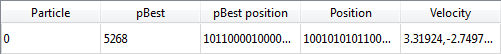
\includegraphics[width=400px]{images/particle.PNG}
    \caption{Particle}
    \label{fig-particle}
\end{figure}

\section{Implementation}
\label{lbl-impl}
This chapter describes the implementation in detail and shows some extracts from the source code. \ref{fig-algo} shows the flow diagram of the implemented algorithm. The single steps and their implementation are outlined in the following sections.

\begin{figure}[H]
    \centering
    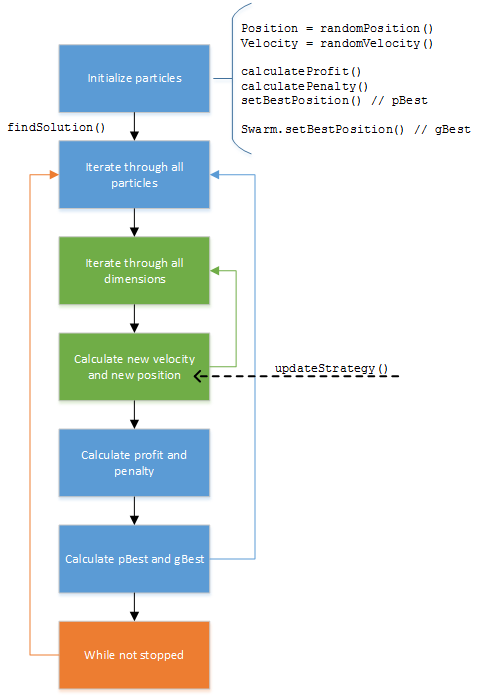
\includegraphics[width=250px]{images/algo.png}
    \caption{Algorithm}
    \label{fig-algo}
\end{figure}

\subsection{Algorithm}
At first, the particles are initialized with random positions and random velocities. After that, the profit of the particular solution is calculated and saved as gBest value. The highest profit of all particles is saved as the swarms gBest value. It is very likely, that the particles have invalid positions, so at this point the penalty values are very high.

\begin{lstlisting}[caption="Solver.cpp"]
for (auto &i : swarm.getParticles()) {
	Solution position = getRandomSolution();
   	Velocity velocity = getRandomVelocity();

	i.setPosition(position);
	i.setVelocity(velocity);
	
	// Fitness value / Profit of the solution/position.
	int profit = calculateProfit(position);
	
	// ... Set gBest and pBest
}
\end{lstlisting}

After initialization, the method \lstinline$findSolution()$ is called, to iterate through all particles of the swarm. For each dimension of the particles the formula \ref{formula-1} and \ref{formula-2} are applied.

\begin{lstlisting}[caption="Solver.cpp"]
double newVelocityD = parameters.getInertiaWeight() *
	currentVelocityD +
	parameters.getConstant1() * randomParticleNumber *
	(pBestD - currentPositionD) +
	parameters.getConstant2() * randomGlobalNumber *
	(gBestD - currentPositionD);

if (newVelocityD > parameters.getVMax())
	newVelocityD = parameters.getVMax();

/* K. and E. */
int newPositionD = updateStrategy_standard(
	currentPositionD, newVelocityD);
\end{lstlisting}

At last, the profit and the penalty values are calculated. With this information the pBest and gBest values can be updated. If the particles current fitness value is higher than its pBest value, the current value is the new pBest. If this is true, this value could be better than the swarms gBest value. So gBest is updated if pBest is higher.

\begin{lstlisting}[caption="Solver.cpp"]
int pBestTmp = calculateProfit(i.getPosition());
pBestTmp -= calculatePenalty(i.getPosition(), pBestTmp);

// Update pBest and gBest position/solution
if (pBestTmp > i.getBestValue()) {
	i.setBestPositionAndValue(i.getPosition(), pBestTmp);
	if (pBestTmp > swarm.getBestValue()) {
	    swarm.setBestPositionAndValue(
	    	i.getPosition(), pBestTmp);
	}
}
\end{lstlisting}

\subsection{Update strategies}
There are several strategies available, to update the particles position based on the velocity. The current used startegie in the implementation is the original strategie from Kennedy and Eberhart \cite{bib-discrete}. A novel based update strategy \cite{bib-novel} and the improved update strategie from Qi Shen are also implemented.

\subsection{Penalty function}
A very important part of the algorithm is the penalty function. Because the knapsack problem has multiple constraints, invalid positions can occur. The penalty function therefore adjusts the fitness value to a valid fitness value (based on several different parameters). There are a many penalty functions to choose from. It is important, to choose a good penalty function, because it does strongly influence the optimization capabilities of PSO. If the penalty function is too weak, invalid positions are more likely and the algorithm does not perform well. If it is too large, it negatively influences the performance of PSO.\\
In this implementation, a penalty function from Oken \cite{bib-penalty} is used. It uses the current fitness value of a particles position to weight the penalty. If a solution has a very large profit and is invalid, it gets a high penalty.

\begin{lstlisting}[caption="Solver.cpp"]
// Check constraint i
int dist = checkConstraint(newPosition, i);

if (dist) {
	// Constraint violated
	
	// ...
	
	// Penalty function
	int penalty = (int) (pBestTmp *
		(((double) dist) / (double) diff));
		
	// Sum up with penalty function
	penaltyValue += penalty;
}
\end{lstlisting}

\subsection{Parameter}
The available parameters are explained in the following table.\\

\begin{tabular}{|l|l|}
	\hline
	Inertia weight ($\omega$) & Specifies the impact of the current velocity to the new velocity \\ \hline
	Constant 1 ($c_1$) & Weights the evidence of the particle \\ \hline
	Constant 2 ($c_2$) & Weights the evidence of the swarm \\ \hline
	Maximal velocity ($V_{max}$) & Limits the velocity \\ \hline
\end{tabular}\\

The best found configuration is displayed in image TODO.

\section{Tests}
\label{lbl-tests}
For the tests, the \lstinline$mknapcb1.txt$ problems from the OR library were used. \\
The very low start values are a result of the penalty function. Because all particles are initialized with random values, it is very likely that the particles violate a constraint and are invalid. Because of that, the particles get a very high penalty. At each iteration, each particles changes it position according to its own current velocity, its own knowledge of the best position and the swarms knowledge of the best position (and some random factors).\\

The following table shows the tests with different parameters.

Picture TODO shows the different particles and its pBest values.

The implemented PSO does converge towards 5\% above the optimum. it does not work optimal, so there are some improvements to do, which are outlined in chapter \ref{lbl-impr}.

\section{Application}
\label{lbl-app}
The application is able to parse files from the OR library with the same format as $mknapcb1.txt$. The GUI   provides tables to view the problems and its values. The user is able to set different parameters via the File-settings dialog. He can choose between automatic or manual (step by step) iteration. Note that the GUI is made only for testing purpose, so there are still some improvements to do. The algorithm is done in the GUI thread, so the GUI blocks (algorithm needs a worker thread).

\begin{figure}[H]
    \centering
    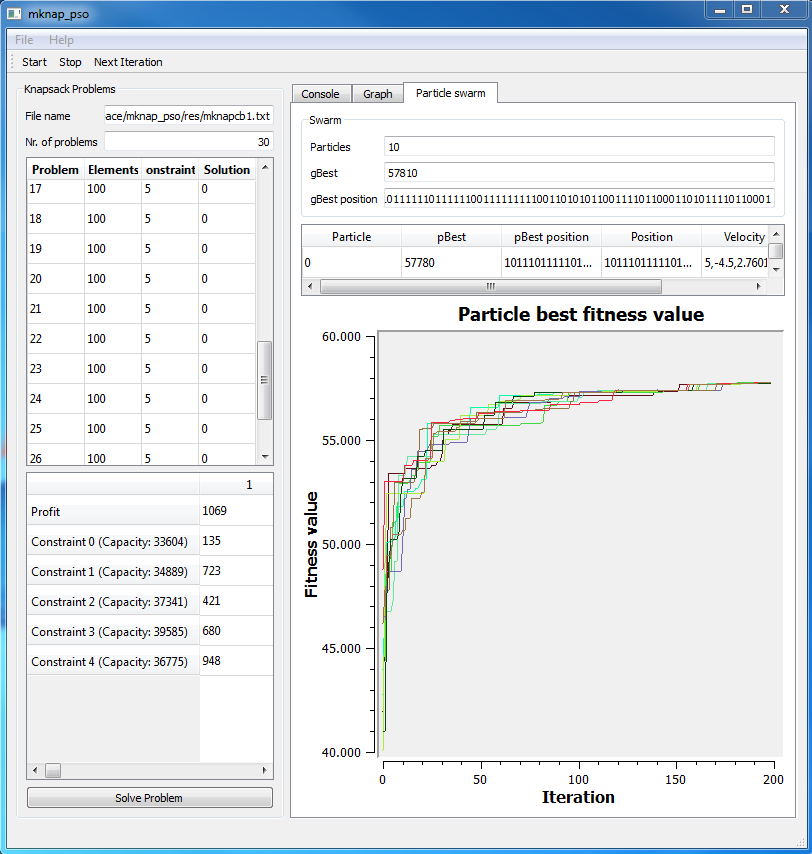
\includegraphics[width=400px]{images/image_main.PNG}
    \caption{Application}
    \label{fig-app}
\end{figure}

\section{Critique and improvements}
\label{lbl-impr}
The discrete PSO does converge towards the optimum, however it does not work optimal. The global best position differs dependent of the problem in average of about 5\% from the optimal value. One problem is the penalty function which could be optimized. It is difficult, to find a suitable penalty function for constrained values. A different approach would be to use TODO. Another optimization is to use a local best position instead of the swarms best position for the calculation of the velocity. In this case, only the $n$ nearest neighbour particles are used to calculate the lBest value.

\newpage

\begin{thebibliography}{99}
	\bibitem{bib-continues}
		Kennedy, J.; Eberhart, R.
		\emph{Particle Swarm Optimization}.
		Proceedings of IEEE International Conference on Neural Networks IV.
		1995
	\bibitem{bib-novel}
		Ling Wang, Xiuting Wang, Jingqi Fu, Lanlan Zhe.
	  	\emph{A Novel Probability Binary Particle Swarm Optimization Algorithm and Its Application}.
	  	JOURNAL OF SOFTWARE, VOL. 3, NO. 9, DECEMBER 2008
	\bibitem{bib-penalty}
		Anne L. Oken.
		\emph{Penalty functions and the knapsack problem}.
		Evolutionary Computation, 1994. IEEE World Congress on Computational Intelligence., Proceedings of the First IEEE Conference on.
	\bibitem{bib-discrete}
		James Kennedy, Russell C. Eberhart.
		\emph{A discrete binary version of the particle swarm algorithm}.
		Systems, Man, and Cybernetics, 1997. Computational Cybernetics and Simulation., 1997 IEEE International Conference on.
\end{thebibliography}

\end{document}